%-------------------------------------------------
%	Version: 0.0
%	fecha de entrega
%
%-------------------------------------------------

\documentclass[11pt]{report}

%packages
\usepackage{graphicx}
\usepackage{subcaption}

\usepackage[utf8]{inputenc}
\usepackage[spanish, es-nodecimaldot]{babel}
\usepackage{setspace}
\usepackage{ragged2e}

\usepackage{amsmath}
\usepackage{amsthm}
\usepackage{amssymb}
\usepackage{mathtools}
\usepackage{siunitx}
\usepackage[thinc]{esdiff} %derivadas faciles
\usepackage{physics} %algunos simbolos de derivadas

%path donde se encuentran las imagenes
\graphicspath{ {./figuras/} }

%---------------------------------------------------------------
%ABREVIACIONES DE COMANDOS

\theoremstyle{plain}
\newtheorem{thm}{Teorema}[chapter] % reset theorem numbering for each chapter

\theoremstyle{definition}
\newtheorem{defn}[thm]{Definición} % definition numbers are dependent on theorem numbers
\newtheorem{exmp}[thm]{Ejemplo} % same for example numbers

\newcommand{\chaptercontent}{
\section{Basics}
\begin{defn}Here is a new definition.\end{defn}
\begin{thm}Here is a new theorem.\end{thm}
\begin{thm}Here is a new theorem.\end{thm}
\begin{exmp}Here is a good example.\end{exmp}
\subsection{Some tips}
\begin{defn}Here is a new definition.\end{defn}
\section{Advanced stuff}
\begin{defn}Here is a new definition.\end{defn}
\subsection{Warnings}
\begin{defn}Here is a new definition.\end{defn}
}

\usepackage{biblatex}
%\addbibresource{Tarea1.bib}

\begin{document}

\begin{titlepage}
\title{Titulo_del_trabajo}

%-------------------------------------------------
%PORTADA
%-------------------------------------------------

	\centering
	{\scshape\LARGE Universidad Autónoma de Yucatán  \\ Facultad de ingeniería\par}
	\vspace{1cm}
	{\scshape\Large Fenómenos de transporte\par}
	\vspace{1.5cm}
	{\huge\bfseries Apuntes de clase\par}
	\vspace{0.7cm}
	{\begin{figure}[!h]
	\centering
    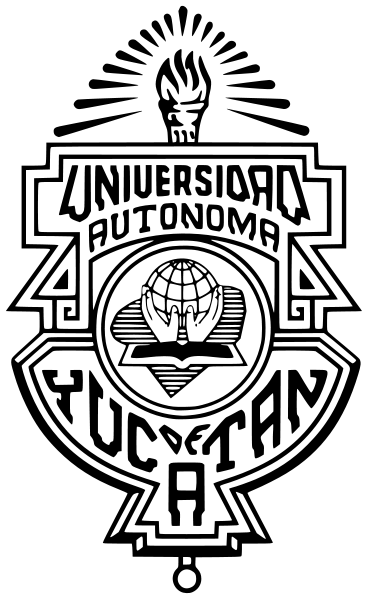
\includegraphics[scale=0.3]{UADY.png}
	\end{figure}}
	\vspace{0.7cm}
	{\Large\itshape Erick Al. Casanova Cortés\par}
	{\Large\itshape Matricula: \par}
	\vfill
	{\scshape\Large Docente\par
	Nombre del docente\par}
	\vfill
	{\Large{\bfseries Fecha de modificacion: \today} }

	\vfill
	
\end{titlepage}

%-------------------------------------------------
%Inicio del documento
%-------------------------------------------------

\tableofcontents

%-------------------------------------------------
%Introducción y conceptos básicos
%-------------------------------------------------
\chapter{Introducción y conceptos básicos}

%---> Formativa <-----
\section{Formativa}
Exámenes (3) 35 \% \\
ADAS (11) 25 \% \\
Proyecto (4) 40 \% \\

\section{Fechas importantes}

Primer parcial 19 abril (conducción) \\
Segundo parcial 3 junio (convección) \\ 
Tercer parcial 1 julio \\

\section{ADAs}
Constan de la resolución de problemas similares a lo que vienen en el examen:\\

\textbf{Características}\\
Carátula escrita en procesador de texto.\\
Resolución de problemas a mano en hojas blancas.\\
Tarea en formato PDF, escaneada con muy buena calidad.\\
Se solicitan y entregan por medio de la plataforma TEAMS.\\
Nombre del archivo ADA\#\_FdT\_CasanovaCortésErickAlejando\\


\section{Proyectos}

\textbf{Primer proyecto}\\
Uso del software Wolfram para determinar el transporte de energía por conducción a nano-escala en ferrofluidos\footnote{Suspensión coloidal estable de nanopartículas de magnetita}.\\


\textbf{Segundo proyecto}\\
Transferencia de calor en estado estacionario en aljibes diatermicos, usando el fusion 360, dibujo de modelos en 3D y simulaciones térmicas.\\


\textbf{Tercer proyecto}\\
Diseño de una madre.\\


\textbf{Cuarto proyecto}\\
Otra shingadera.\\


%-------------------------------------------------
%Conducción de calor
%-------------------------------------------------
\chapter{Conducción de calor}

%-------------------------------------------------
%Introducción a la conducción del calor
\section{Introducción a la conducción del calor}


%-------------------------------------------------
%La termodinamica y la transferencia de calor
\subsection{La termodinamica y la transferencia de calor}

La termodinámica se interesa en la cantidad de calor de un estado a otro. La transferencia de calor se enfoca en la dinámica misma del transporte de energía.

El requisito básico para la transferencia de calor (TC) es la presencia de una diferencia de temperatura. A mayor gradiente de temperatura, mayor razón de la TC.

Podría decirse que FdT es la derivada con respecto del tiempo de la termodinámica.

Fundamentos históricos:

Se decía que el calórico era una sustancia que no se podía crear ni destruir. ¿Cómo refutaría la teoría del calórico?

1a ley de termodinámica -> conservación de la energía\\
2a ley de termodinámica -> entropía del univ aumenta\\
Ley 0 de termodinámica -> equilibrio térmico\\
3ra ley de termodinámica -> no se puede llegar al 0 abs\\


Normalmente para resolver problemas complejos es requerido visualizar el parámetro más importante, para así poder elaborar un modelo de la transferencia de calor. 

\subsection{Calor y otras formas de energía} %%%%%%%%

La energía puede existir en numerosas formas: térmica, mecánica, cinemática, potencial, eléctrica... \\

También existe energía sensible o calor sensible: está asociada a la energía cinética de las moléculas.\\
El calor latente está energía con la fase de un sistema.\\
Energía química es la energía asociada con los enlaces atómicos de las moléculas.\\
Energía nuclear está asociada con los enlaces en el interior del núcleo.\\


Entalpía: combinación entre la energía interna y el trabajo de flujo (Pv) en un fluido.\\

Recordar que para un gas ideal se cumple:
\begin{equation}
	Pv = RT
	\label{eq:gas_ideal}
\end{equation}



\subsection{Mecanismos de transferencia de calor} %%%%%%%%
La termodinámica se interesa en la cantidad de calor transferido.\\
La ciencia que trata de la razón a la cual se mueve esa energía es la transferencia de calor.\\

Los mecanismos de transferencia de calor son tres:
\begin{enumerate}
	\item conducción
	\item convección
	\item radiación
\end{enumerate}


\subsection{Conducción} %%%%%%%%

La conducción es la transferencia de energía de las partículas más energéticas de una sustancia hacia las adyacentes menos energéticas, como resultado de interacciones entre esas partículas

La razón de la conducción de calor a través de una capa plana es proporcional a la diferencia de temperatura a través de esta y al área de transferencia de calor pero inversamente proporcional al espesor de esa capa es decir:

\begin{equation*}
	\dot{Q}_{\text{cond}} = kA\frac{T_1 - T_2}{\Delta X}
\end{equation*}

Ley de Fourier de la conducción del calor:
\begin{equation*}
	\dot{Q}_{\text{cond}} = -kA\frac{\dd{T}}{\dd{x}}
\end{equation*}

\subsection{Difusivilidad termica}

Habla de que tan rápido se difunde el calor por un material, la cual puede verse como:
\begin{equation*}
	\alpha = \frac{\text{calor conducido}}{\text{calor almacenado}}
\end{equation*}


Ley de enfriamiento de Newton

A pesar de la complejidad de la convección, se observa que la rapidez de la transferencia de calor por convección es proporcional a la diferencia de temperatura y se expresa en forma conveniente por la ley de Newton de enfriamiento como

\begin{equation}
	\dot{Q}_\text{conv} = hA_s(T_s-T_\infty)
	\label{eq:ley_enfriamiento_newton}
\end{equation}

\subsection{Radiación}

Es la energía emitida por la materia en forma de ondas electromagnéticas o fotones, como resultado de los cambios de las configuraciones de los átomos o moléculas. A diferencia de la conducción y la convección, la radiación no requiere de un medio

\begin{equation}
	\dot{Q}_\text{conv, max} = \sigma A_s T^4_s
	\label{eq:radiación}
\end{equation}


También está la radiación por cuerpos grises, la emisividad que está de 0 a 1, es una medida en cuán próxima está una superficie de ser un cuerpo negro, para el cual la emisividad es $\varepsilon = 1$.


Otra importante propiedad es la absortividad, 

%-------------------------------------------------
%Conducción de calor en es estado estacionario
\section{Conducción de calor en es estado estacionario}


%-------------------------------------------------
%Conducción de calor en régimen transitorio
\section{Conducción de calor en régimen transitorio}


%-------------------------------------------------
%Convección de calor
%-------------------------------------------------
\chapter{Convección de calor}
%-------------------------------------------------
%
\section{Fundamentos de la convección}
%-------------------------------------------------
%
\section{Convección externa forzada}
%-------------------------------------------------
%
\section{Conveccón interna forzada}
%-------------------------------------------------
%
\section{Ebullición y condensación}


%-------------------------------------------------
%Radiación de calor
%-------------------------------------------------
\chapter{Radiación de calor}
%-------------------------------------------------
%
\section{Fundamentos de la radiación}
%-------------------------------------------------
%
\section{Transferencia de calor por radiación}


%-------------------------------------------------
%Transferencia de masa
%-------------------------------------------------
\chapter{Transferencia de masa}
%-------------------------------------------------
%
\section{Introducción}
%-------------------------------------------------
%
\section{Difusión de masa}
%-------------------------------------------------
%
\section{Convección de masa}
%-------------------------------------------------
%
\section{Transferencia simultanea de calor y masa}


%-------------------------------------------------
%Final del documento
%-------------------------------------------------

\end{document}
